\documentclass[a4paper]{article}
\usepackage[utf8]{inputenc}
\usepackage[T1]{fontenc}
\usepackage[finnish]{babel}
\usepackage{geometry}
\usepackage{graphicx}
\usepackage{url}

\usepackage{color}
\usepackage{hyperref}
\hypersetup{
    colorlinks=true, % make the links colored
    linkcolor=black, % color TOC links in blue
    urlcolor=red, % color URLs in red
    linktoc=all % 'all' will create links for everything in the TOC
}


\begin{document}
\begin{titlepage}
\begin{center}
\section*{Tietokantasovelluksen harjoitustyö}
\begin{LARGE}
{DRINKKIARKISTO}
\end{LARGE}
\linebreak
\linebreak
\begin{large}
Emma Kämäräinen
\end{large}
\linebreak
\linebreak
Kevät 2015

\end{center}


\end{titlepage}



\tableofcontents

\section{Johdanto}

Harjoitustyön aiheena drinkkiarkisto. Tarkoituksena on luoda drinkkireseptejä sisältävä www-sivusto. Sivuustoon kirjaudutaan sisään. Kirjautunut käyttäjä voi olla joko ylläpitäjä tai sitten tavallinen käyttäjä. Ylläpitäjällä on mahdollisuus lisätä ylläpito-oikeudet tavalliselle käyttäjälle.   

Kirjautumisen jälkeen sivustolla voi selailla juoma-reseptejä, tutkia reseptien tietosivuja ja halutessaan lisätä juoman. Juomaan lisätään ainesosia yksi kerrallaan juoman tietosivulta. Jos ainesosa on jo olemassa, sitä ei lisätä tietokantaan. Myös kaikki tietokannassa olevat juomien ainesosat ovat selailtavissa omalla sivullaan. 

Mikäli kirjautuneella käyttäjällä on ylläpito-oikeudet, on hänen mahdollista nähdä myös käyttäjistä koostuva selailusivu. Tämän sivun  kautta ylläpitäjällä on mahdollisuus antaa muille käyttäjille ylläpito-oikeuksia. Jokainen käyttäjä pystyy muokkaamaan omia käyttäjätietojaan ja halutessaan poistaa itsensä sivustolta. 

Tietokantana on PostgreSQL. Harjoitustyö toteutetaan laitoksen user--palvelimella PHP-kielellä. 

\newpage
\section{Käyttäjistä}

\subsection{Käyttötapauskaavio}
\begin{figure}[h]
	
	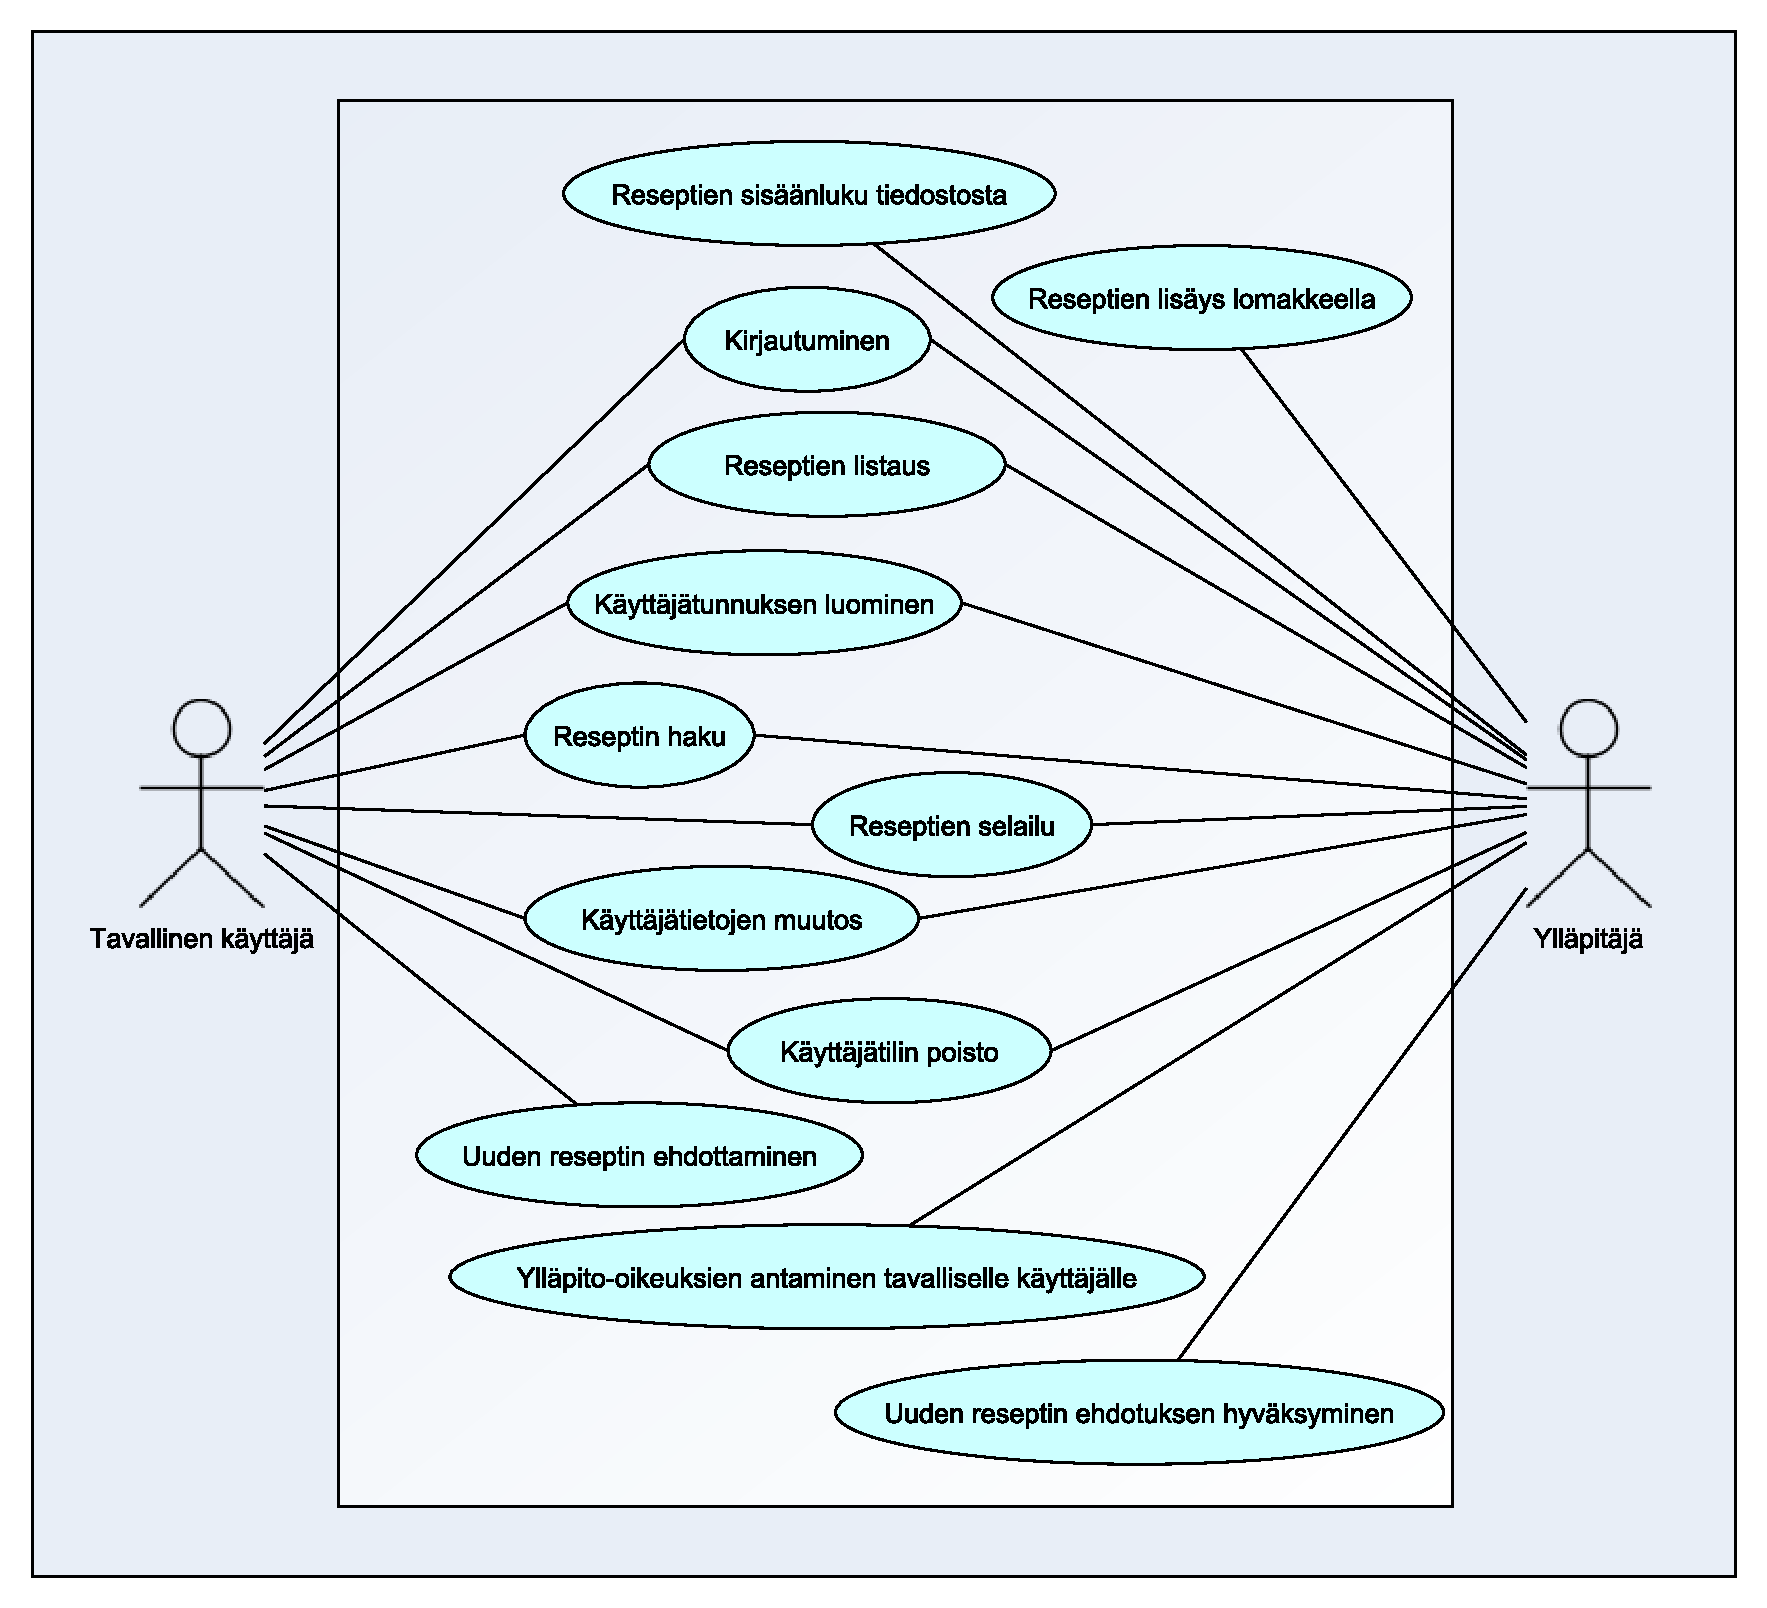
\includegraphics[scale=0.9]{kayttotapaukset.pdf}
	\caption{Käyttötapauskaavio}
\end{figure}
	
\subsection{Käyttäjäryhmät}

\begin{flushleft}Ylläpitäjä\end{flushleft}
\begin{itemize}
\item Ylläpitäjän pitää olla rekisteröitynyt sivuston käyttäjä, jolle on annettu ylläpito-oikeudet. Sivusto vaatii sisäänkirjautumisen.
\end{itemize}
\begin{flushleft}Tavallinen käyttäjä\end{flushleft}
\begin{itemize}
\item Tavallinen käyttäjä voi olla kuka tahansa sivulle kirjautunut henkilö. 
\end{itemize}

\newpage
\subsection{Käyttötapaukset}

\begin{flushleft}\textbf{Ylläpitäjä\(\colon\)} \end{flushleft}
\begin{itemize}
	\item Reseptien listaus\(\colon\) käyttäjä voi listata reseptit.
	\item Reseptin lisäys\(\colon\) käyttäjä voi lisätä reseptin käyttäen siihen tarkoitettua lomaketta. 
	\item Reseptin poisto\(\colon\) ylläpitäjä voi poistaa juomareseptin.
	\item Ainesosien listaus\(\colon\) käyttäjä voi listata reseptien ainesosat.
	\item Ainesosien lisääminen juomaan\(\colon\) käyttäjä voi lisätä juomaan ainesosia lomakkeella.
	\item Ylläpito-oikeuden antaminen tavalliselle käyttäjälle\(\colon\) käyttäjä voi tehdä tavallisesta käyttäjästä ylläpitäjän.
	\item Käyttäjien listaus\(\colon\) ylläpitäjä voi listata sivuston käyttäjät.
	\item Muut käyttötapaukset\(\colon\) Käyttäjätietojen muutos, käyttäjätilin poisto, käyttäjätunnuksen luominen, kirjautuminen
\end{itemize}

\begin{flushleft}\textbf{Tavallinen käyttäjä\(\colon\)} \end{flushleft}

\begin{itemize}
		\item Reseptien listaus\(\colon\) käyttäjä voi listata reseptit.
	\item Reseptin lisäys\(\colon\) käyttäjä voi lisätä reseptin käyttäen siihen tarkoitettua lomaketta. 
	\item Ainesosien listaus\(\colon\) käyttäjä voi listata reseptien ainesosat.
	\item Ainesosien lisääminen juomaan\(\colon\) käyttäjä voi lisätä juomaan ainesosia lomakkeella.
	\item Muut käyttötapaukset\(\colon\) Käyttäjätietojen muutos, käyttäjätilin poisto, käyttäjätunnuksen luominen, kirjautuminen
\end{itemize}

\newpage
\section{Järjestelmän tietosisältö}
\subsection{Käsitekaavio}

\includegraphics[scale=0.8]{kasitekaavio.pdf}

\subsection{Tietokohde: Juoma}
\begin{flushleft}
	\begin{tabular}{|l|l|l|}\hline
			Attribuutti      & Arvojoukko        & Kuvailu\\
			\hline
			nimi & merkkijono, maksimissaan 50 merkkiä & Juoman nimi.\\ 
			\hline		
			lisäyspäivämäärä & päivämäärä (date) & Päivämäärä, jolloin drinkkiohje on lisätty.\\ 
			\hline			
			juomalaji    & merkkijono,maksimissaan 50 merkkiä  & Juoman käyttötarkoitus. \\ 
			\hline
			kuvaus    & merkkijono, maksimissaan 400 merkkiä & Juoman kuvaus. \\ 
				\hline
	\end{tabular}
\end{flushleft}

\subsection{Tietokohde: Ainesosat}
\begin{flushleft}
	\begin{tabular}{|l|l|l|}
			\hline
			Attribuutti & Arvojoukko & Kuvailu \\ 
			\hline
			ainesosa & merkkijono, maksimissaan 50 merkkiä & Ainesosan nimi. \\ 
			\hline
	\end{tabular}
\end{flushleft}

\subsection{Tietokohde: Käyttäjä}
\begin{flushleft}
	\begin{tabular}{|l|l|l|}
			\hline
			Attribuutti & Arvojoukko & Kuvailu   \\ 
			\hline
			nimimerkki  & merkkijono, maksimissaan 50 merkkiä & Käyttäjän nimimerkki. \\ 
			\hline
			salasana    & merkkijono, maksimissaan 50 merkkiä & Käyttäjän salasana.   \\ 
			\hline
			ylläpitäjä    & boolean & Kertoo onko käyttäjä ylläpitäjä.   \\
			\hline
	\end{tabular}
\end{flushleft}

\subsection{Tietokohde: Juoma-aineyhteys}
\begin{flushleft}
	\begin{tabular}{|l|l|l|}
			\hline
			Attribuutti & Arvojoukko & Kuvailu   \\ 
			\hline
			juoma id  & lukujono & Yhteys Juoma-tauluun. \\ 
			\hline
			ainesosa id    & lukujono & Yhteys Ainesosa-tauluun.  \\ 
			\hline
	\end{tabular}
\end{flushleft}

\section{Relaatiokaavio}
\begin{flushleft}\textbf{Relaatiokaavio} \end{flushleft}

\includegraphics[scale=0.8]{relaatiokaavio.pdf}


\section{Järjestelmän yleisrakenne}

Kansiorakenne tulee melkein suoraan forkatusta reposta. ”App”-kansioon on sijoitettu alakansioita, 
joissa sijaitsevat samoilla nimillä kontrollerit, mallit ja näkymät. Näkymät on jaettu vielä alakansioihin 
sisällön mukaan (juoma, user ja aine). Base.html-nimisessä näkymässä on nähtävissä navigaatiopalkin html-koodaus. Malleista (models) löytyvät pääluokat juoma, user ja aine. Dokumentaatio 
sijaitsee kansiossa ”doc”. Sieltä löytyvät tähän sovellukseen liittyvät kaaviot ja ohjeet. Tietokantasovellusta
tehdessä on käytetty MVC-mallia. 

Sovellukseen kirjaudutaan, joka käynnistää session. Kirjautunut käyttäjä näkee listaukset, pystyy lisäämään juoman ja muokkaamaan 
drinkkiohjeita. Kirjautunut käyttäjä pystyy myös muokkaamaan omia käyttäjätietojaan tai niin halutessaan poistamaan käyttäjätunnuksensa. Ylläpitäjä pystyy korottamaan tavallisen käyttäjän ylläpitäjäksi. Ylläpitäjä pystyy poistamaan muita käyttäjiä. Vain ylläpitäjä kykenee poistamaan lisätyn juomareseptin. Sovelluksesta voi kirjautua ulos, jolloin palaa takaisin etusivulle. 



\newpage
\section{Käyttöliittymä ja järjestelmän komponentit}
\begin{flushleft}\textbf{Käyttöliittymä ja järjestelmän komponentit} \end{flushleft}

\includegraphics[scale=0.8]{sivunakymat.pdf}

\section{Asennustiedot}

Sovelluksen tiedostot ovat tällä hetkellä users-palvelimella htdocs-hakemistossa, josta ne voi halutessaan kopioida.

Harjoitustyö löytyy osoitteesta \url{http://kaem.users.cs.helsinki.fi/Drinkkiarkisto/}


\section{Käynnistys- /käyttöohje}

Sovellukseen pitää kirjautua sisään. Kirjautumaton käyttäjä ei voi tehdä sivulla oikeastaan mitään. Kirjautunut käyttäjä voi olla joko tavallinen käyttäjä tai sitten ylläpitäjä. Ylläpitäjä näkee enemmän sisältöä sivuilla kuin tavallinen käyttäjä, muun muassa käyttäjäselailusivun.

Kirjautumissivulle pääsee joko etusivulta, tai sitten yläpalkin kautta. Kirjautumaton käyttäjä päätyy vain kirjautumissivulle, vaikka hän painaisi yläpalkissa mitä tahansa. Kirjautumisen jälkeen näkymät muuttuvat. Yläpalkissa on linkit ”Drinkkiarkisto”, joka johtaa etusivulle, ”Juomat”, joka johtaa kaikkien juomareseptien listaussivulle, ja ”Aineet”, joka listaa juomien ainesosat omaksi listakseen. Ylläpitäjä näkee myös listan sovelluksen käyttäjistä. Käyttäjien listaussivulta pääse ylläpitojen antamissivulle. Kirjautuneen käyttäjän yläpalkissa on myös käyttäjätiedot, josta näkee omat käyttäjätietonsa, ja linkki uloskirjautumiseen.

Ylläpitäjän näkymää pääsee katsomaan käyttäjätunnuksella ”admin” ja sen salasanalla ”admin”. Tavallisen käyttäjän sivut aukeavat puolestaan tunnuksilla ”kayttaja” ja sitä vastaavalla salasanalla ”kayttaja”.

\section{Testaus, tunnetut bugit ja puutteet ja jatkokehitysideat}
Olisin halunnut toteuttaa vielä ainakin juomareseptien haun joko reseptien nimen perusteella tai sitten ainesosan nimellä, mutta aika ei riittänyt. Myöskin olisi ollut kiva tehdä parempi listaus juomien ainesosille: ainesosan nimeä painaessa olisi näkynyt missä juomissa ainesosa on. Myös tällä hetkellä ainesosa voi olla listassa, vaikka se ei kuulu mihinkään juomaan, ja se on ehkä hieman tyhmää. Demossa toisella samasta aiheesta tehneellä oli myös juomakohtaiset valmistusohjeet (ja ainesosien määrät), mutta nämä eivät jostain syystä tulleet minulle mieleen aikaisemmin enkä ehdi niitä enää lisätä. Jos tämä olisi oikea, käytössä oleva juomareseptiarkisto, niin ne pitäisi tietysti lisätä. 

Sivustoa testatessa huomasin, että jos muokkaussivuilla tekee liian monta virhettä peräkkäin, päätyy "404 Page not found"-sivulle. Liittynee jotenkin siihen, että polusta häviää muokattavan drinkin/käyttäjän tunnus. Lisäksi juoman lisäyksessä on mahdollista tällä hetkellä lisätä sama juoma monta kertaa.  Myöskin rekisteröityessä käyttäjäksi on mahdollista ottaa sama nimimerkki kuin jollain muulla. Korjaisin nämä jos olisi enemmän aikaa. 

En tehnyt sovellukselle testausta, sillä sitä ei vaadittu eikä olisi oikein ollut aikaakaan.

\section{Omat kokemukset}
Harjoitustyön alussa olin kyllä aivan pihalla. Tuntuu, että näinä viikkoina vastaan on tullut sekalaisesti asiaa, joista osa on jäänyt hieman sumeaksi mielikuvaksi. Itselläni meni monta viikkoa, ennenkuin tajusin mallien, sivunäkymien, routesin ja kontrollereiden yhteyden. Kovasti tuntui, että kooditoteutukseni oli aikalailla samaa kuin materiaalissa ja jos materiaalissa ei jotain ollut painittu (kuten miten ylläpitäjän näkymät luodaan), niin ei sitä osannut itse oikein lähteä ajattelemaan. Tuntuu myös, että vieläkin koodissa on kohtia joita en ymmärrä. Mutta samaan aikaan tämän sovelluksen tekeminen on ollut kivaa, on hienoa nähdä miten saa asioita toimimaan ja pystyy lisäämään ja poistamaan tietokannasta asioita. Ehkäpä olisi tarvinnut enemmän aikaa, jotta olisi pystynyt kunnolla sisäistämään, mitä oikein on tekemässä ja tutkimaan erilaisia toteutusvaihtoehtoja (kuin ne jotka materiaalissa suoraan annettiin). 

Iso kiitos pajaohjaajille, taisin valehtelematta olla aina paikalla ja kiva että jaksoitte auttaa välillä kovin tyhmissäkin ongelmissa! :)

\section{Muu dokumentaatio}

SQL--luontitaulut löytyät repositiostani sql-kansiosta.

\end{document}
